\section*{Appendix A. Confusion Matrix}

\begin{figure}[ht]
  \centering
   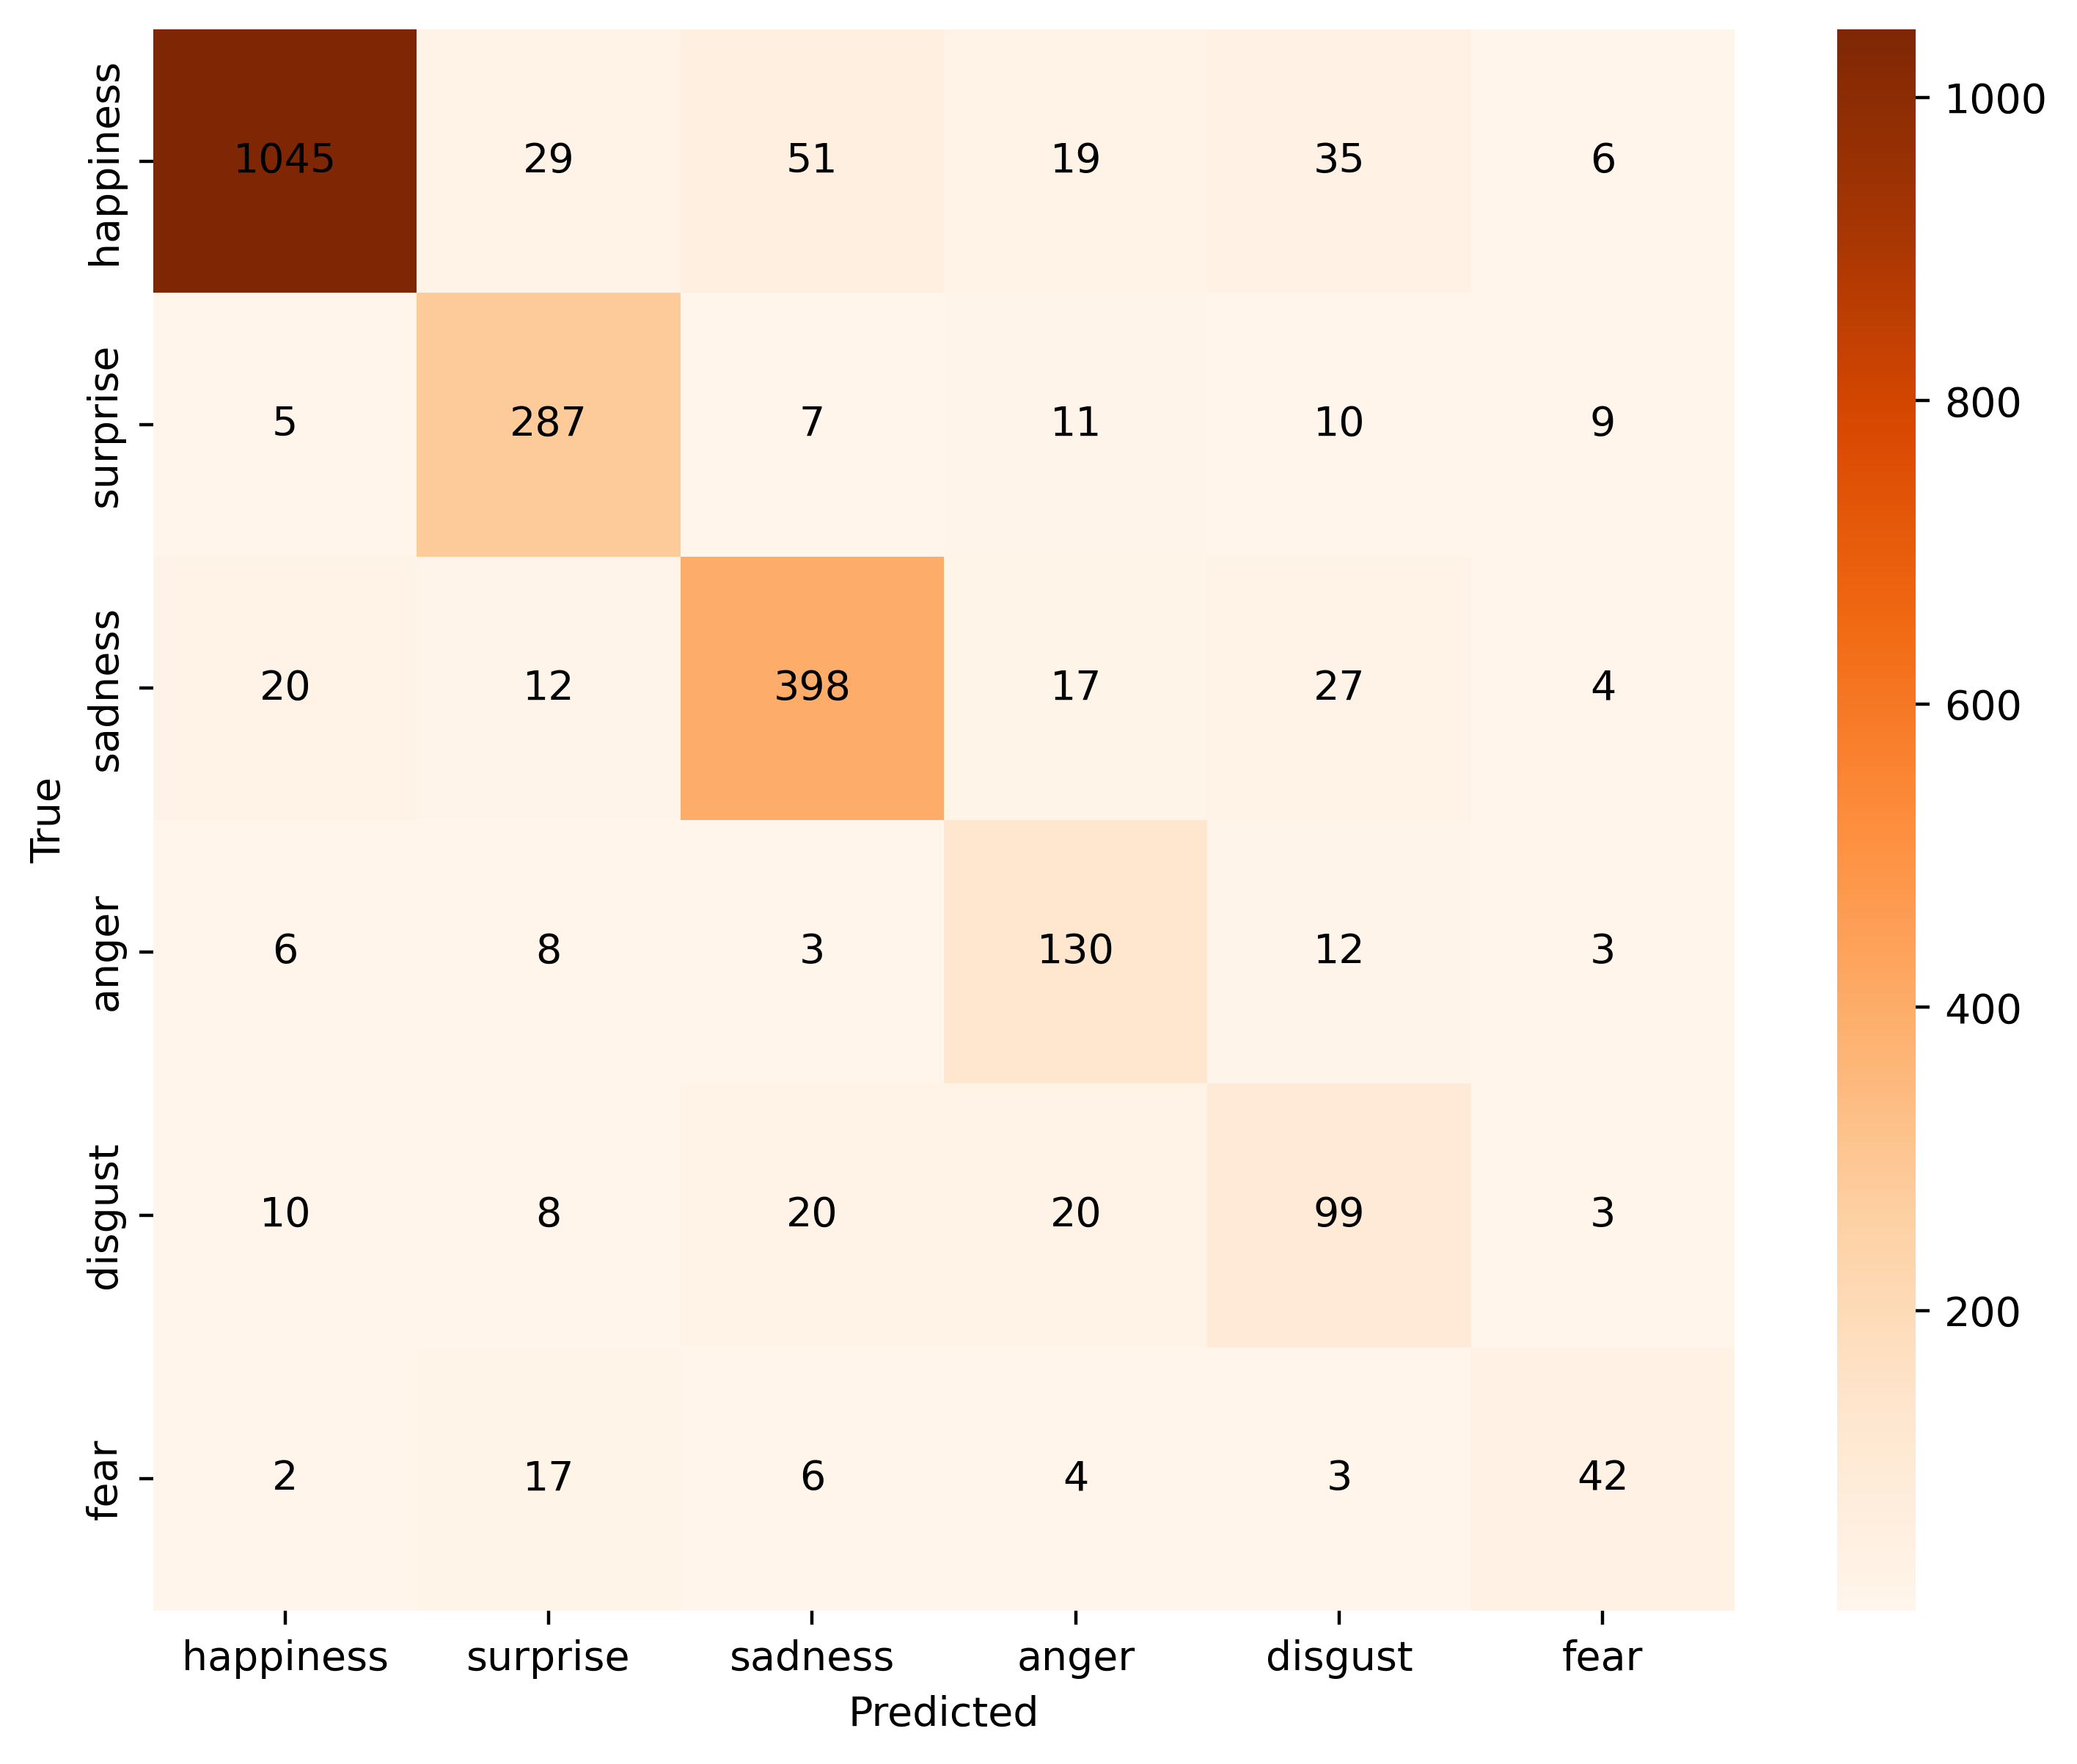
\includegraphics[width=\linewidth]{mattest.png}
   \caption{Overview of the confusion matrix on the test set of RAF-DB.} 
   \label{fig:mattest}
\end{figure}

\newpage 

\section*{Appendix B. Model Architecture}

\tikzstyle{layer} = [rectangle, rounded corners, minimum width=3cm, minimum height=0.8cm,text centered, draw=black, fill=LightPurple!30]
\tikzstyle{pool} = [rectangle, rounded corners, minimum width=3cm, minimum height=0.8cm, text centered, draw=black, fill=cvprblue!30]
\tikzstyle{fc} = [rectangle, minimum width=3cm, minimum height=0.8cm, text centered, draw=black, fill=Orange!30]
\tikzstyle{do} = [rectangle, minimum width=3cm, minimum height=0.8cm, text centered, draw=black, fill=LMUGrey2!30]
\tikzstyle{arrow} = [thick,->,>=stealth]
% \tikzset{arrow/.style={thick,-{Stealth[length=10mm,width=2mm]}}}

\begin{figure}[ht]
  \centering
  \resizebox{.143\textwidth}{!}{
  \begin{tikzpicture}[node distance=1.7cm]

    \node (input) [layer] {Input $3 \times H \times W$};
    \node (conv1) [layer, below of=input] {Conv1 $64$, $3\times3$, padding=1};
    \node (bn1) [layer, below of=conv1] {BatchNorm1 $64$};
    \node (pool1) [pool, below of=bn1] {MaxPool $2\times2$};
    \node (dropout1) [do, below of=pool1] {Dropout $0.2$};
    \node (conv2) [layer, below of=dropout1] {Conv2 $128$, $3\times3$, padding=1};
    \node (bn2) [layer, below of=conv2] {BatchNorm2 $128$};
    \node (pool2) [pool, below of=bn2] {MaxPool $2\times2$};
    \node (dropout2) [do, below of=pool2] {Dropout $0.2$};
    \node (conv3) [layer, below of=dropout2] {Conv3 $256$, $3\times3$, padding=1};
    \node (bn3) [layer, below of=conv3] {BatchNorm3 $256$};
    \node (pool3) [pool, below of=bn3] {MaxPool $2\times2$};
    \node (dropout3) [do, below of=pool3] {Dropout $0.2$};
    \node (conv4) [layer, below of=dropout3] {Conv4 $512$, $3\times3$, padding=1};
    \node (bn4) [layer, below of=conv4] {BatchNorm4 $512$};
    \node (pool4) [pool, below of=bn4] {MaxPool $2\times2$};
    \node (dropout4) [do, below of=pool4] {Dropout $0.2$};
    \node (conv5) [layer, below of=dropout4] {Conv5 $1024$, $3\times3$, padding=1};
    \node (bn5) [layer, below of=conv5] {BatchNorm5 $1024$};
    \node (pool5) [pool, below of=bn5] {MaxPool $2\times2$};
    \node (adaptivePool) [pool, below of=pool5] {AdaptiveAvgPool};
    \node (fc1) [fc, below of=adaptivePool] {FC1 $2048$};
    \node (dropout6) [do, below of=fc1] {Dropout $0.5$};
    \node (fc2) [fc, below of=dropout6] {FC2 $1024$};
    \node (fc3) [fc, below of=fc2] {FC3 $6$};

    \draw [arrow] (input) -- (conv1);
    \draw [arrow] (conv1) -- (bn1);
    \draw [arrow] (bn1) -- (pool1);
    \draw [arrow] (pool1) -- (dropout1);
    \draw [arrow] (dropout1) -- (conv2);
    \draw [arrow] (conv2) -- (bn2);
    \draw [arrow] (bn2) -- (pool2);
    \draw [arrow] (pool2) -- (dropout2);
    \draw [arrow] (dropout2) -- (conv3);
    \draw [arrow] (conv3) -- (bn3);
    \draw [arrow] (bn3) -- (pool3);
    \draw [arrow] (pool3) -- (dropout3);
    \draw [arrow] (dropout3) -- (conv4);
    \draw [arrow] (conv4) -- (bn4);
    \draw [arrow] (bn4) -- (pool4);
    \draw [arrow] (pool4) -- (dropout4);
    \draw [arrow] (dropout4) -- (conv5);
    \draw [arrow] (conv5) -- (bn5);
    \draw [arrow] (bn5) -- (pool5);
    \draw [arrow] (pool5) -- (adaptivePool);
    \draw [arrow] (adaptivePool) -- (fc1);
    \draw [arrow] (fc1) -- (dropout6);
    \draw [arrow] (dropout6) -- (fc2);
    \draw [arrow] (fc2) -- (fc3);

  \end{tikzpicture}
  }
  \caption{Overview of our detailed model architecture.} 
  \label{fig:modeldetail}
\end{figure}

\tikzstyle{line} = [draw, -latex', line width=0.7pt]


% \begin{figure}[ht]
%   \centering
%   \resizebox{.47\textwidth}{!}{
%   \begin{tikzpicture}[
%     node distance=1cm,
%     auto,
%     rect/.style={rectangle, draw=black, align=center, thick, minimum height=1.5cm, minimum width=2.7cm},
%     box/.style={rectangle, rounded corners, draw=black, align=center, thick, minimum height=1.5cm, minimum width=3cm},
%     bigbox/.style={rectangle, rounded corners, draw=LMUGreen, thick, inner sep=0.3cm, line width=1pt, fill=LMUGreen!5} 
%   ]
%     \node [rect] (data) {Data};
%     \node [rect, below=of data] (mlmodel) {ML Model};
%     \node [rect, below=of mlmodel] (preds) {Predictions};
%     \node [box, right=of mlmodel, fill=cvprblue!30] (interpretability) {Interpretability};
%     \node [box, right=of interpretability, fill=LightPurple!30] (inspection) {Human Inspection};
%     \node [box, below=of inspection] (predictions) {Verified Predictions};

%     \begin{pgfonlayer}{background}
%       \node[bigbox, fit=(data) (mlmodel) (preds)] (group) {};
%     \end{pgfonlayer}
    
%     \path [line] (data) -- (mlmodel);
%     \path [line] (mlmodel) -- (preds);
%     \path [line] (mlmodel) -- (interpretability);
%     \path [line] (interpretability) -- (inspection);
%     \path [line] (inspection) |- node[below left] {Data Improvement} (data);
%     \path [line] (inspection) -- node[left] {Model Improvement}  (predictions);

%   \end{tikzpicture}
%   }
%   \caption{Overview of the traditional standardized ML evaluation process 
%   (see the illustration in the large \textcolor{LMUGreen}{green} box) and the explainable AI pipeline} 
%   \label{fig:xai}
% \end{figure}


% \begin{figure*}[ht]
%   \centering
%   \begin{subfigure}{0.32\linewidth} % 0.24
%     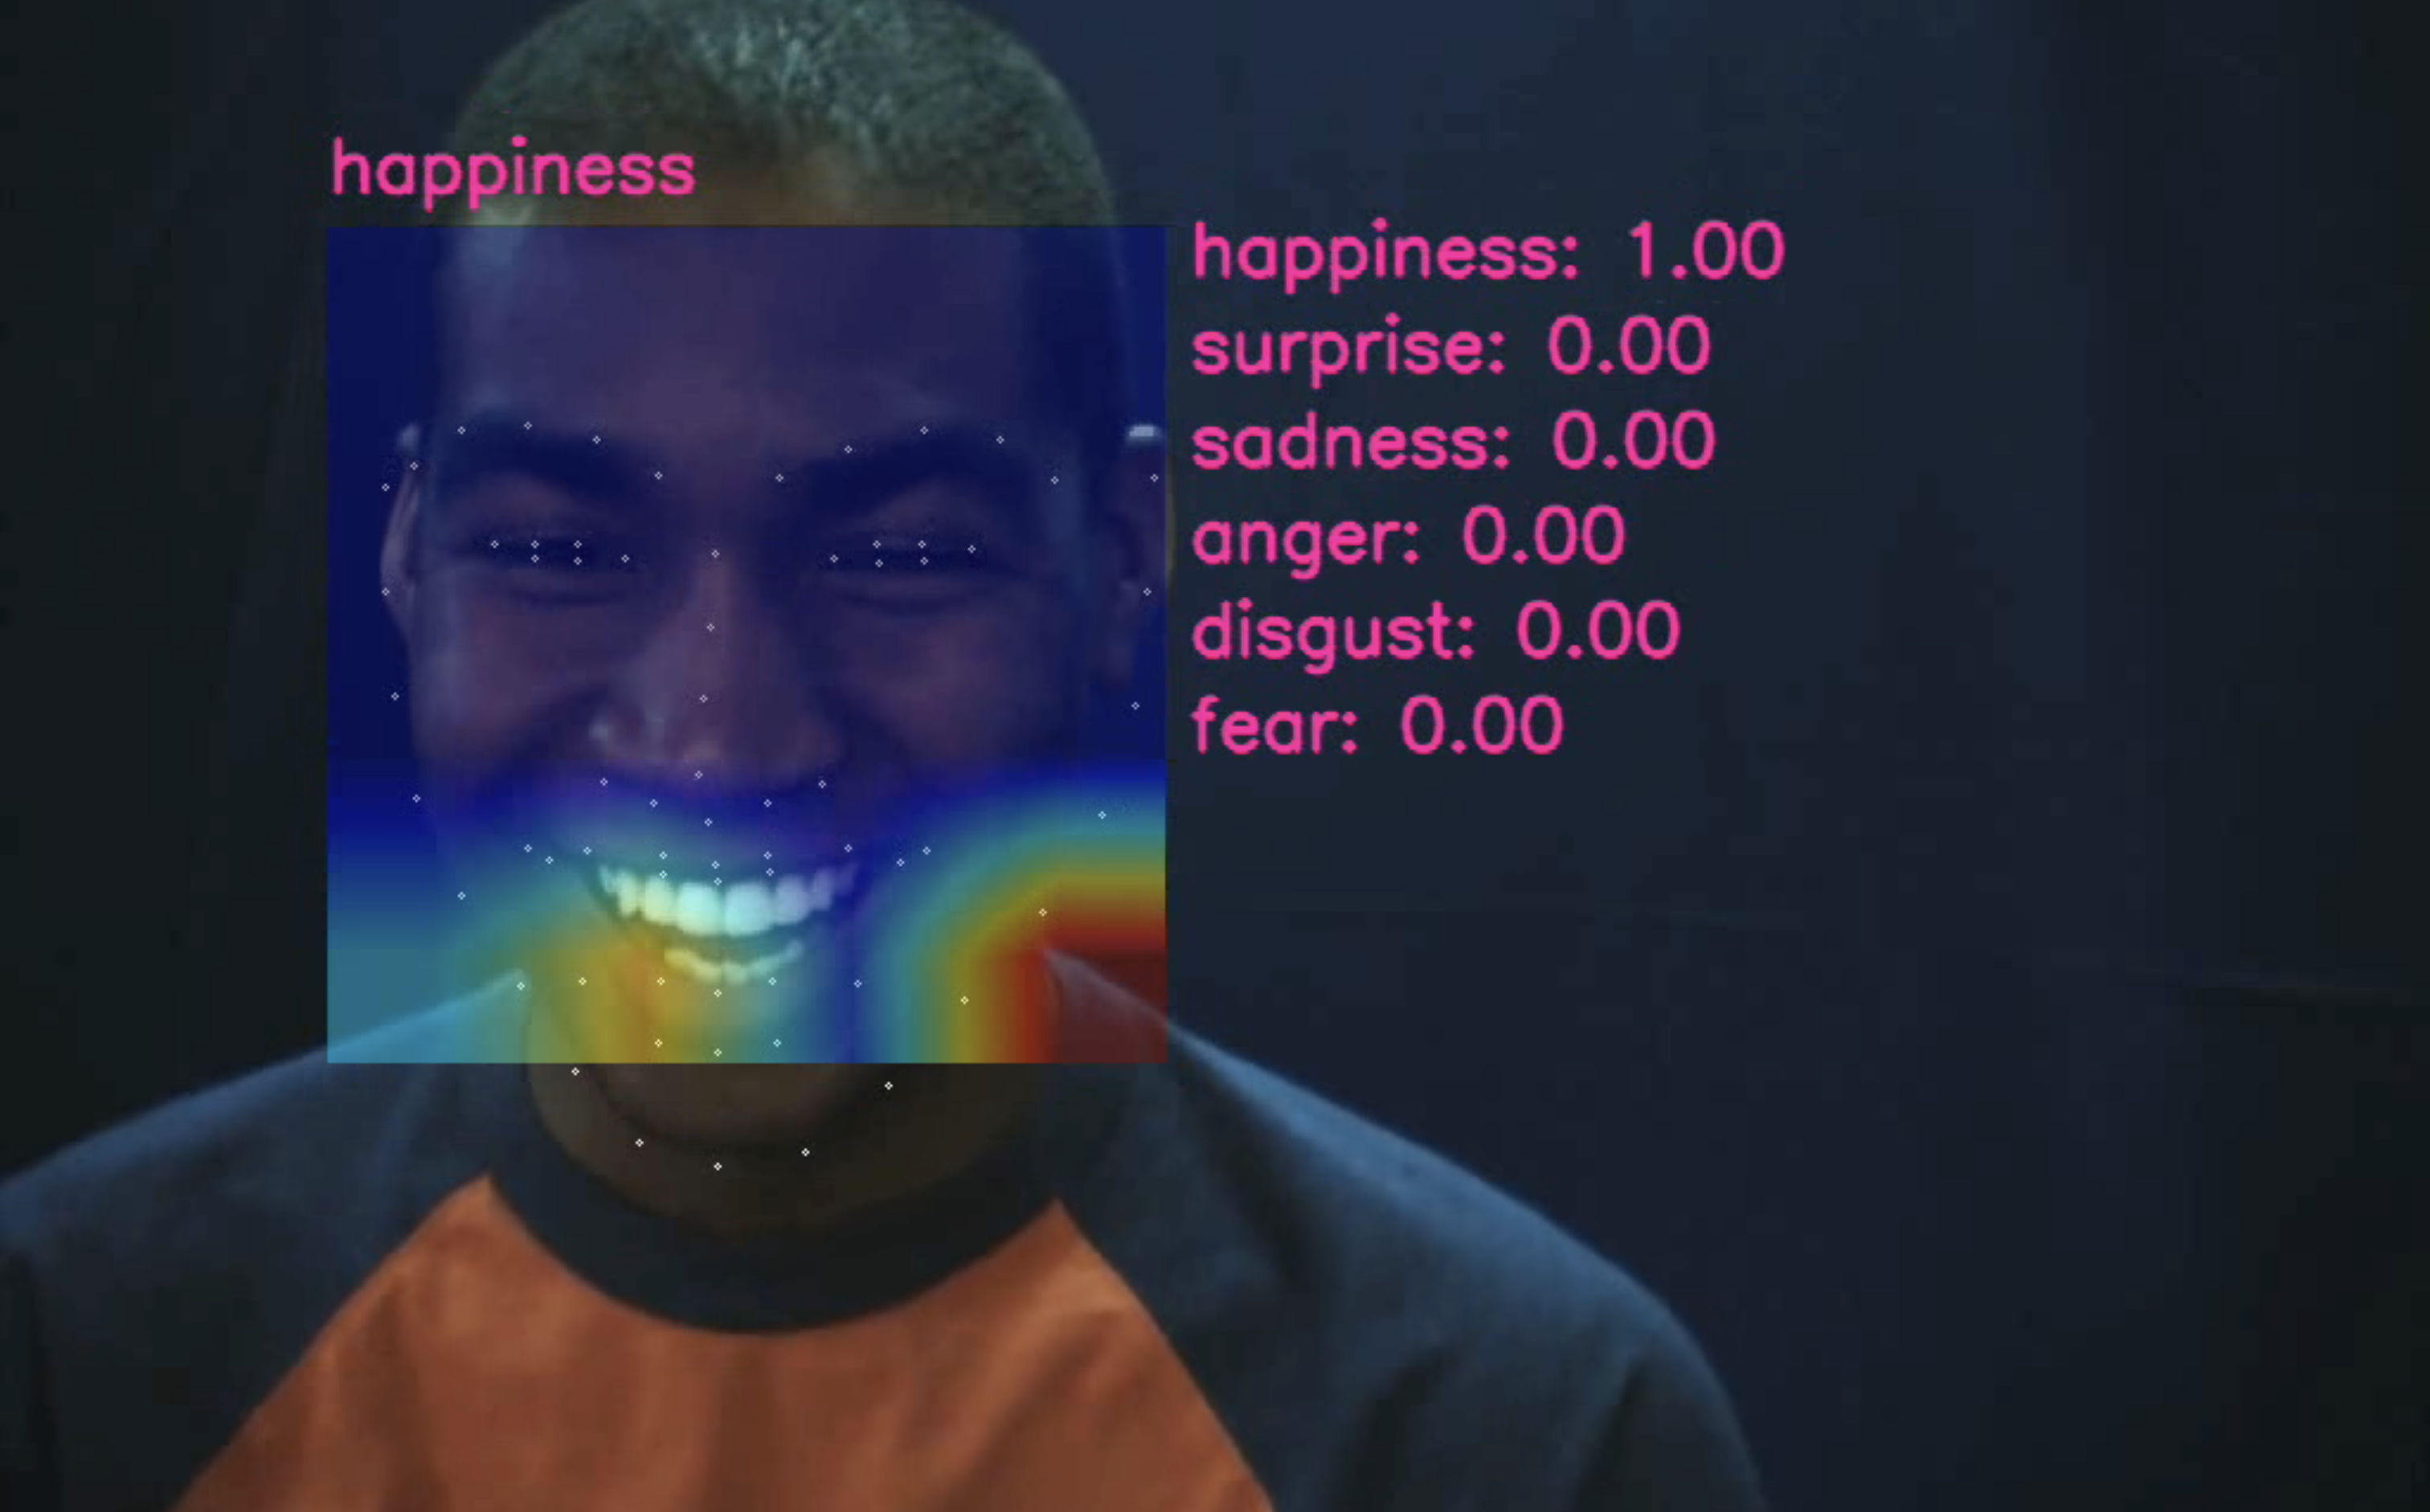
\includegraphics[width=\linewidth]{video/v_happiness.png}
%     \caption{Happiness.}
%     \label{fig:v1}
%   \end{subfigure}
%   \hfill
%   \begin{subfigure}{0.32\linewidth}
%     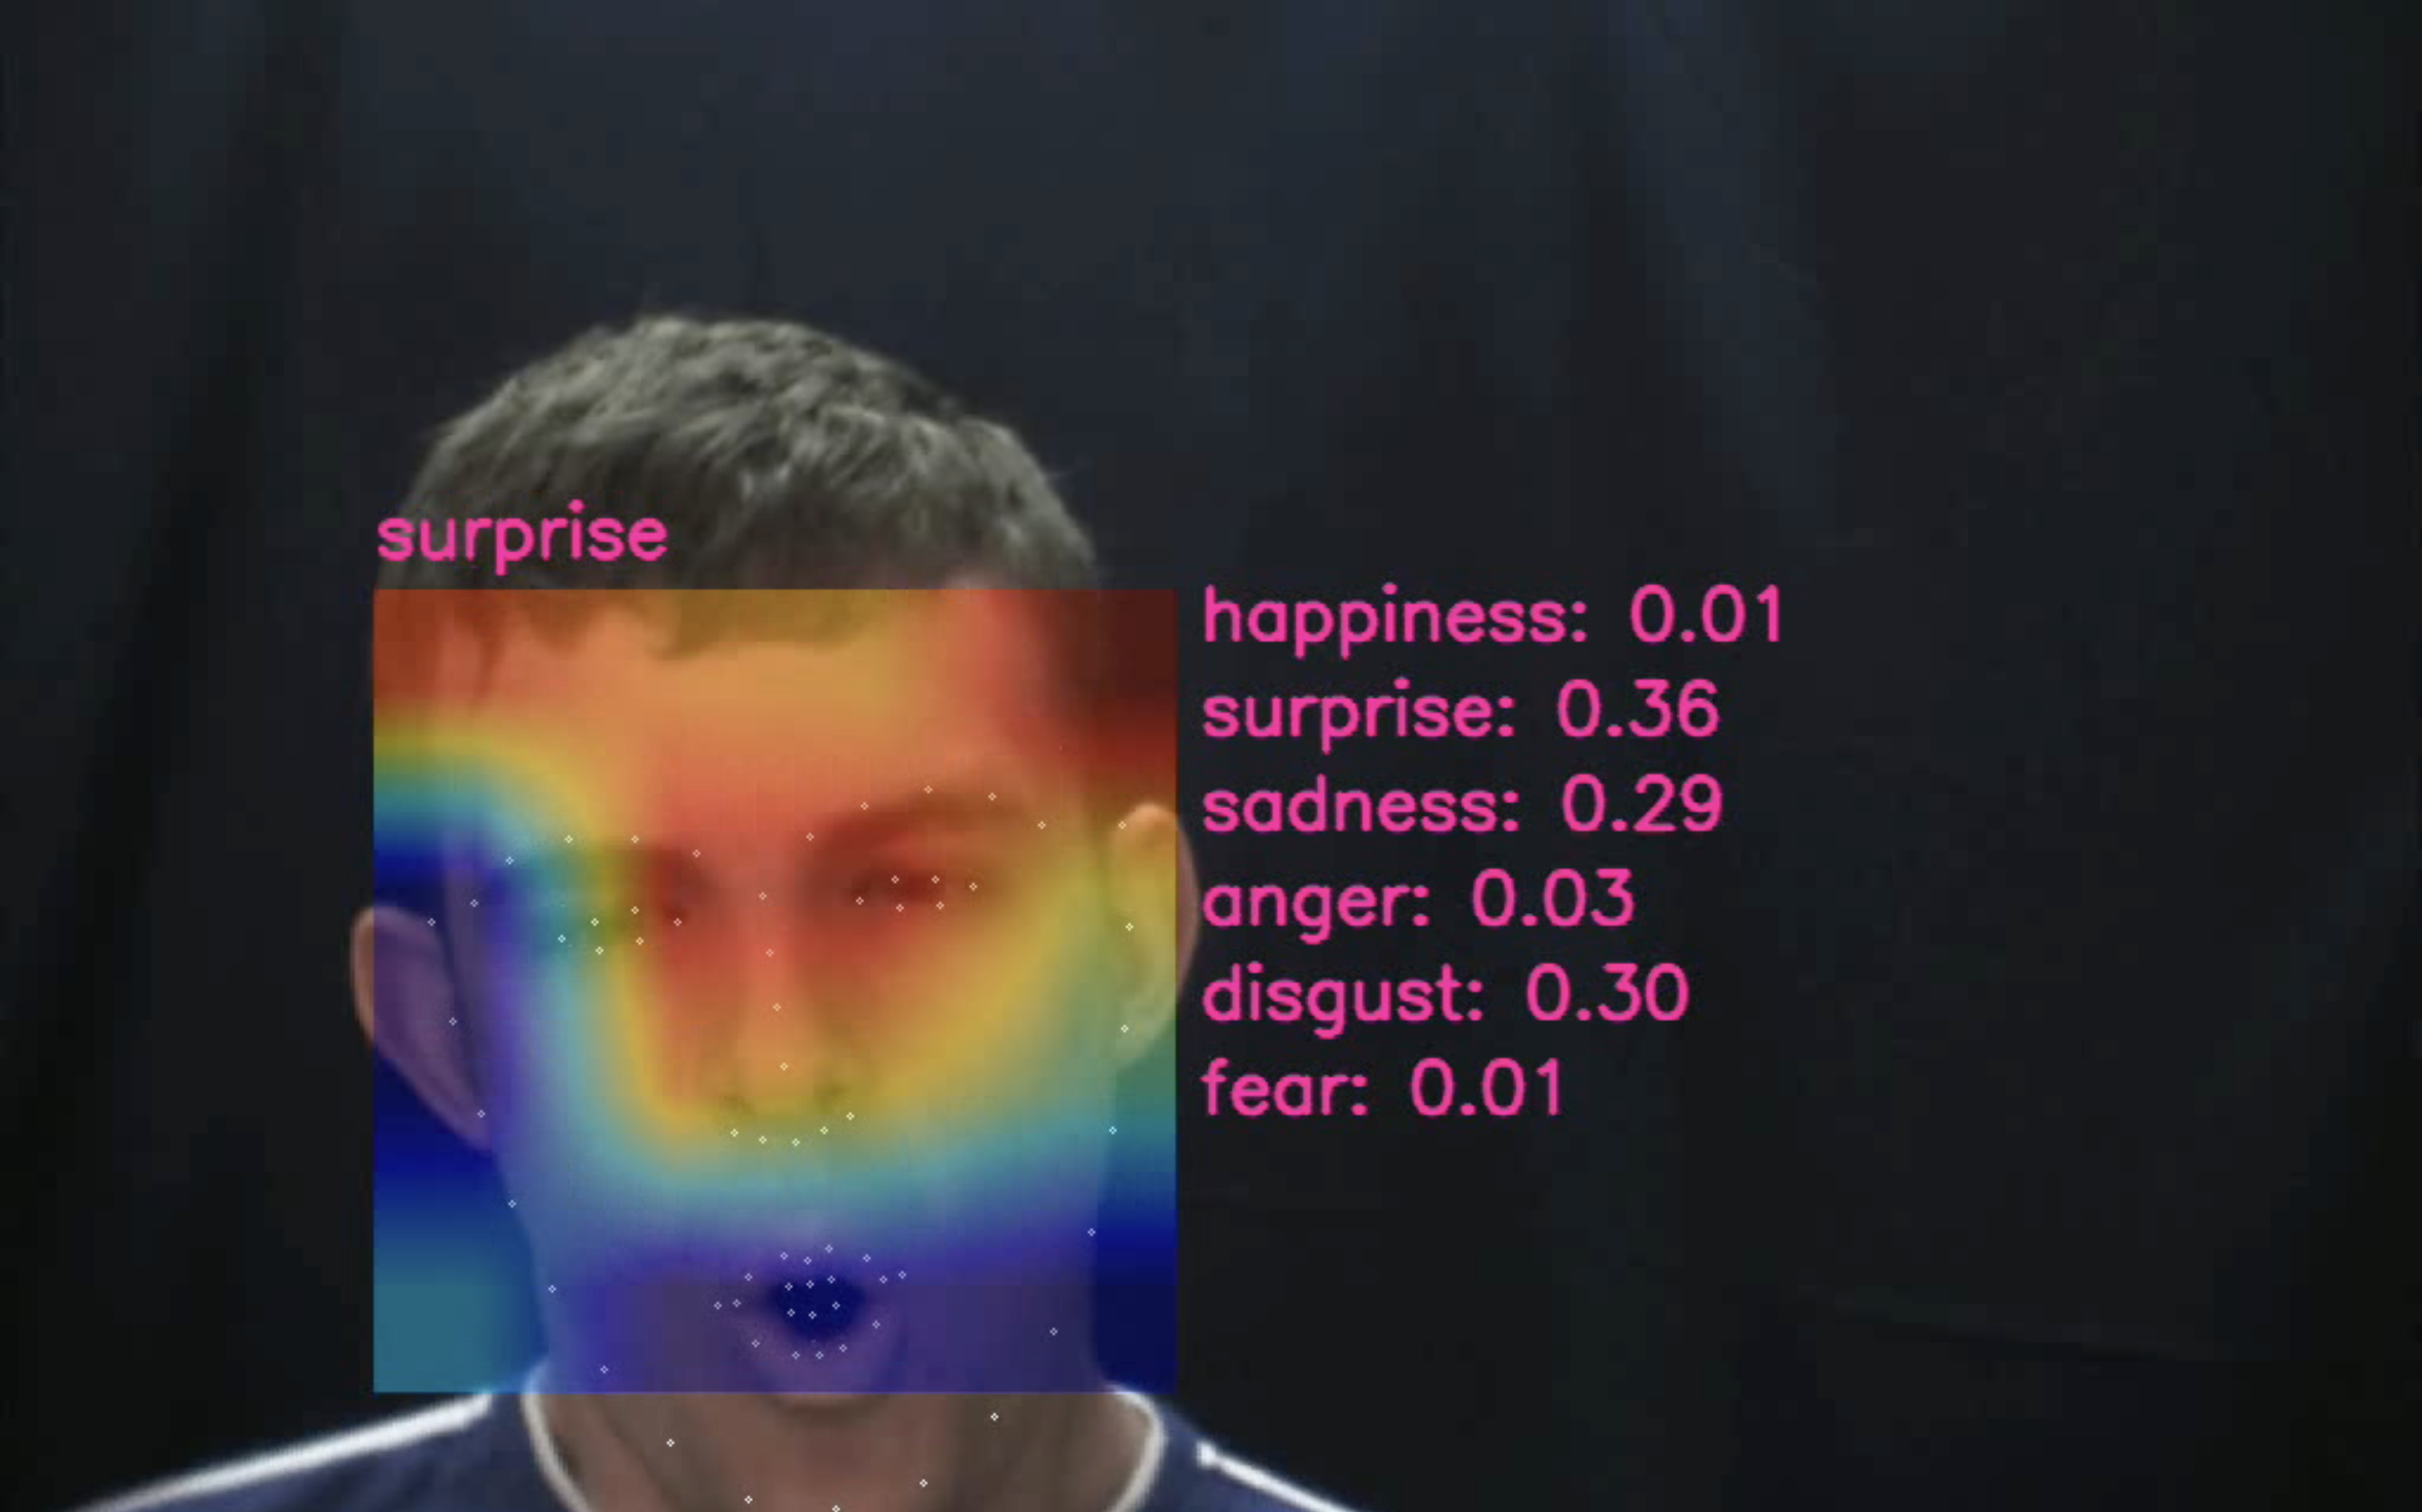
\includegraphics[width=\linewidth]{video/v_surprise.png}
%     \caption{Fear.}
%     \label{fig:v2}
%   \end{subfigure}
%   \hfill
%   \begin{subfigure}{0.32\linewidth}
%     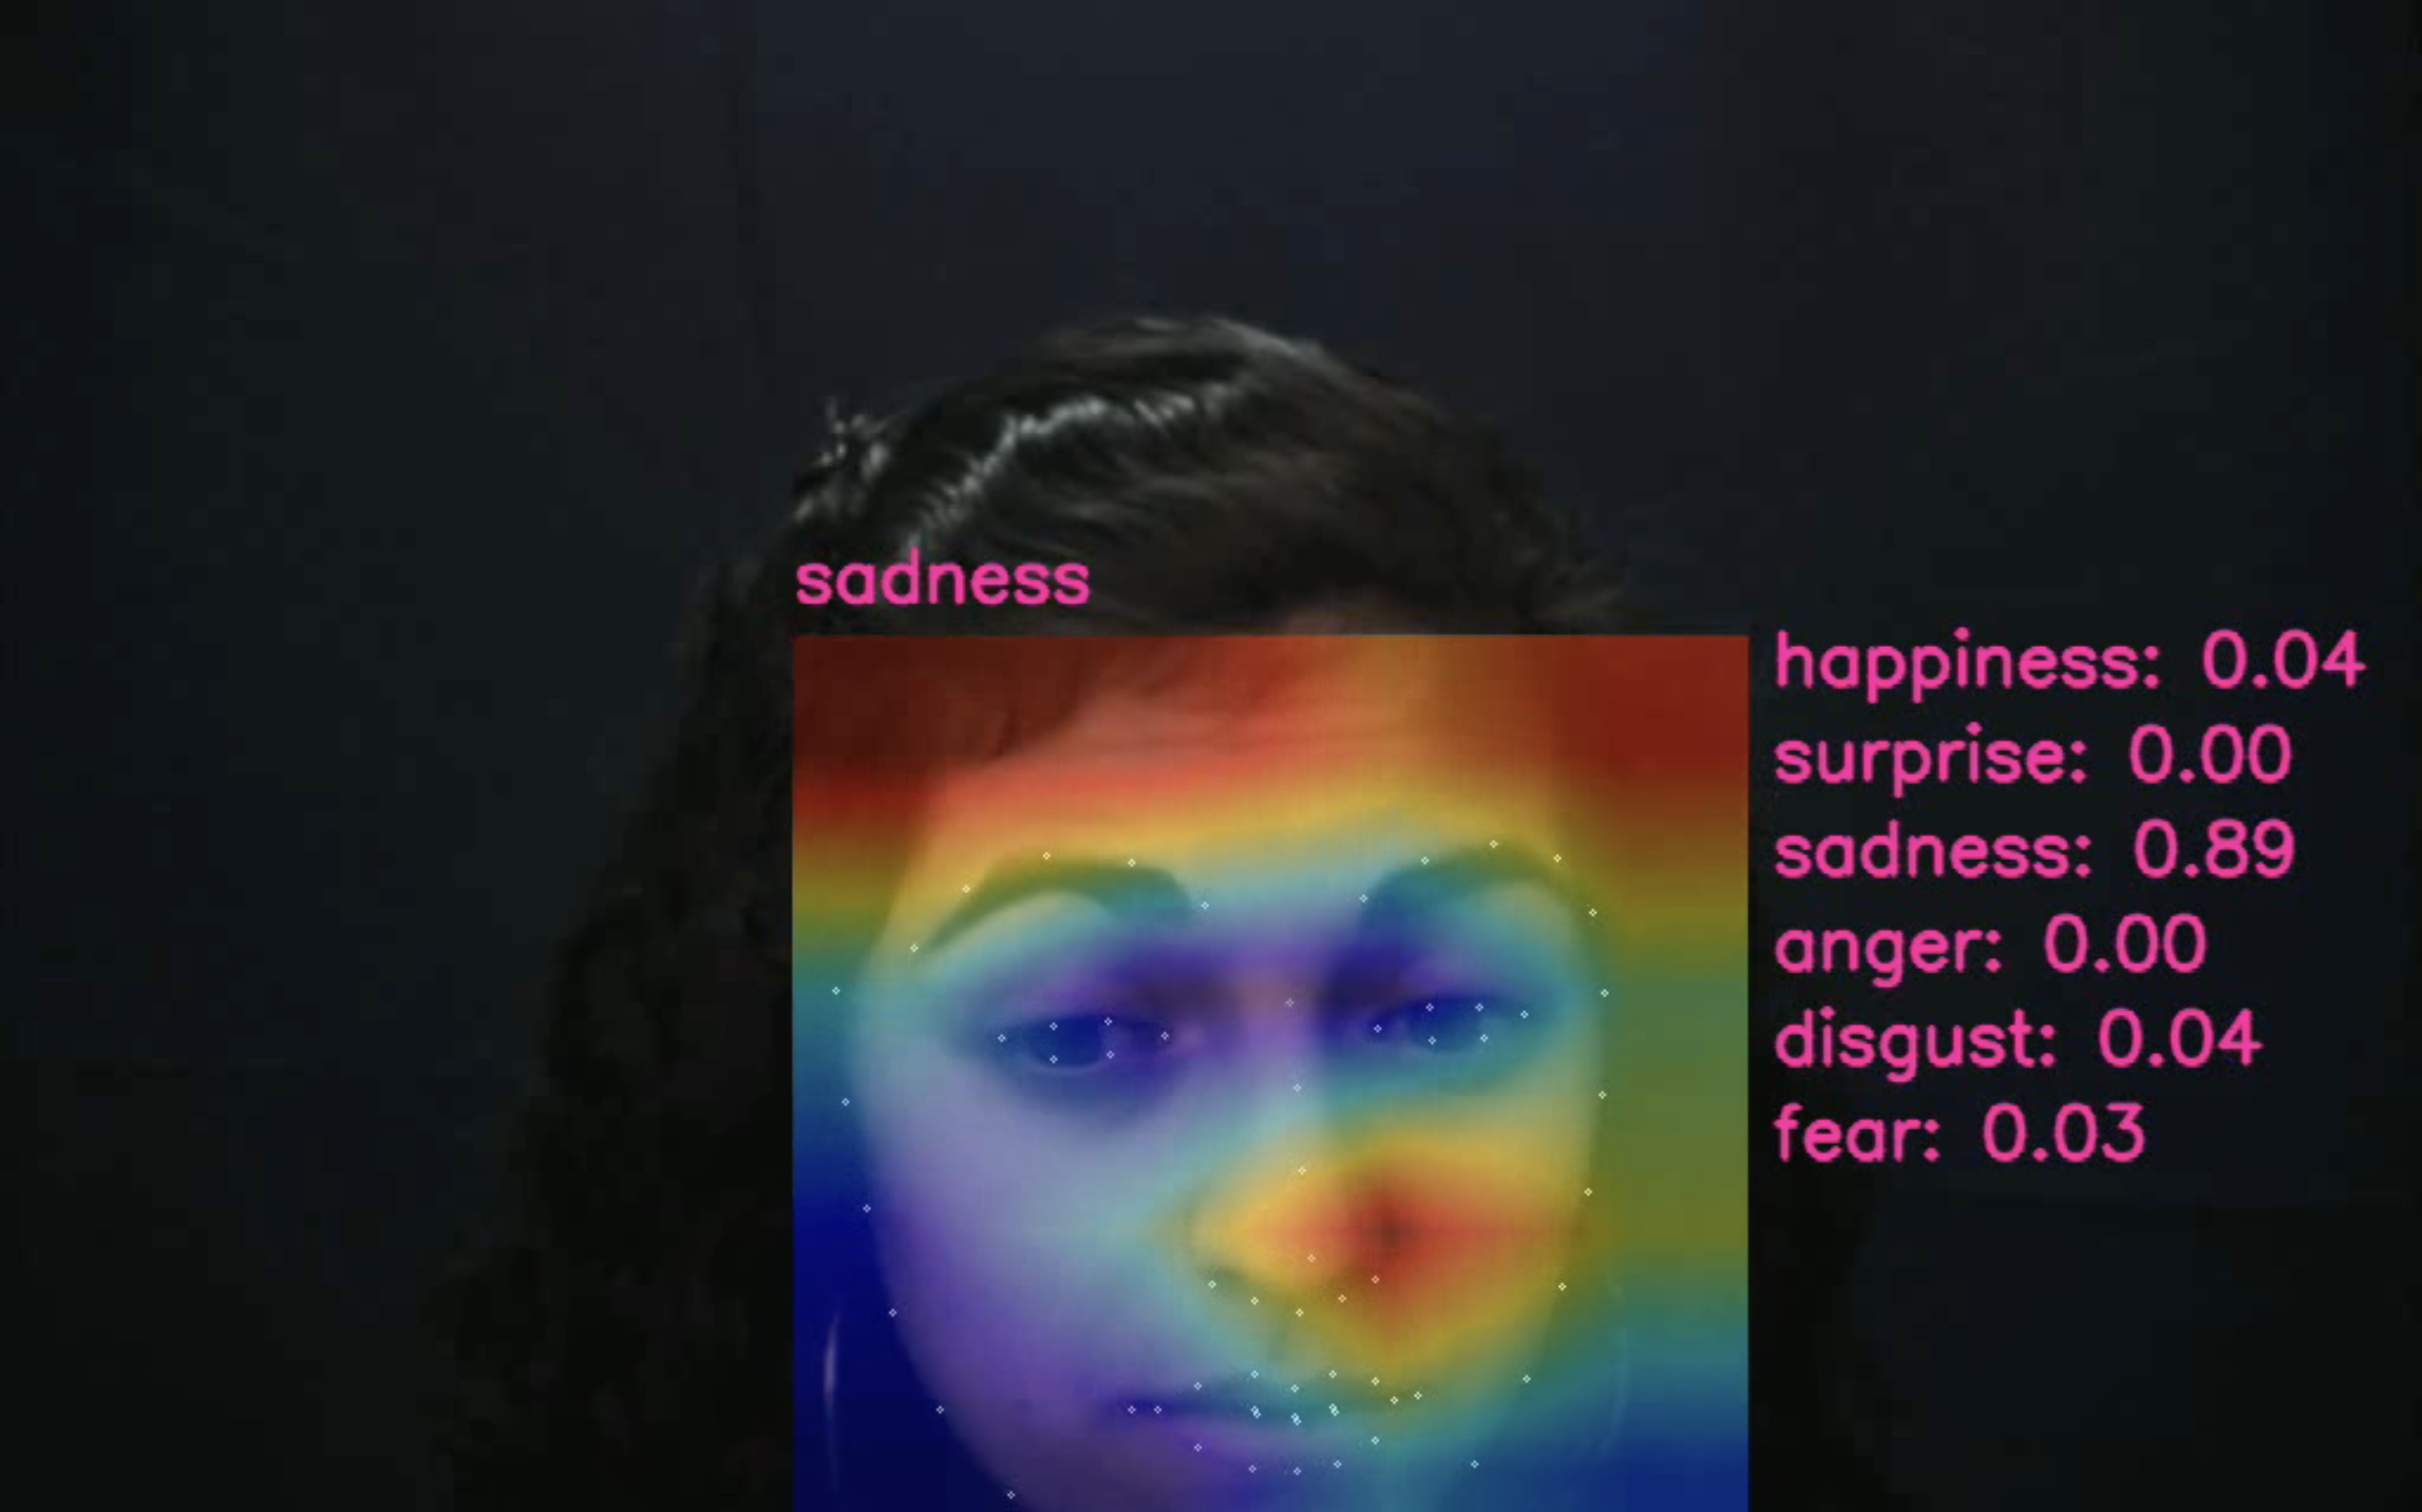
\includegraphics[width=\linewidth]{video/v_sadness.png}
%     \caption{Surprise.}
%     \label{fig:v3}
%   \end{subfigure}
%   \hfill
%   \begin{subfigure}{0.32\linewidth}
%     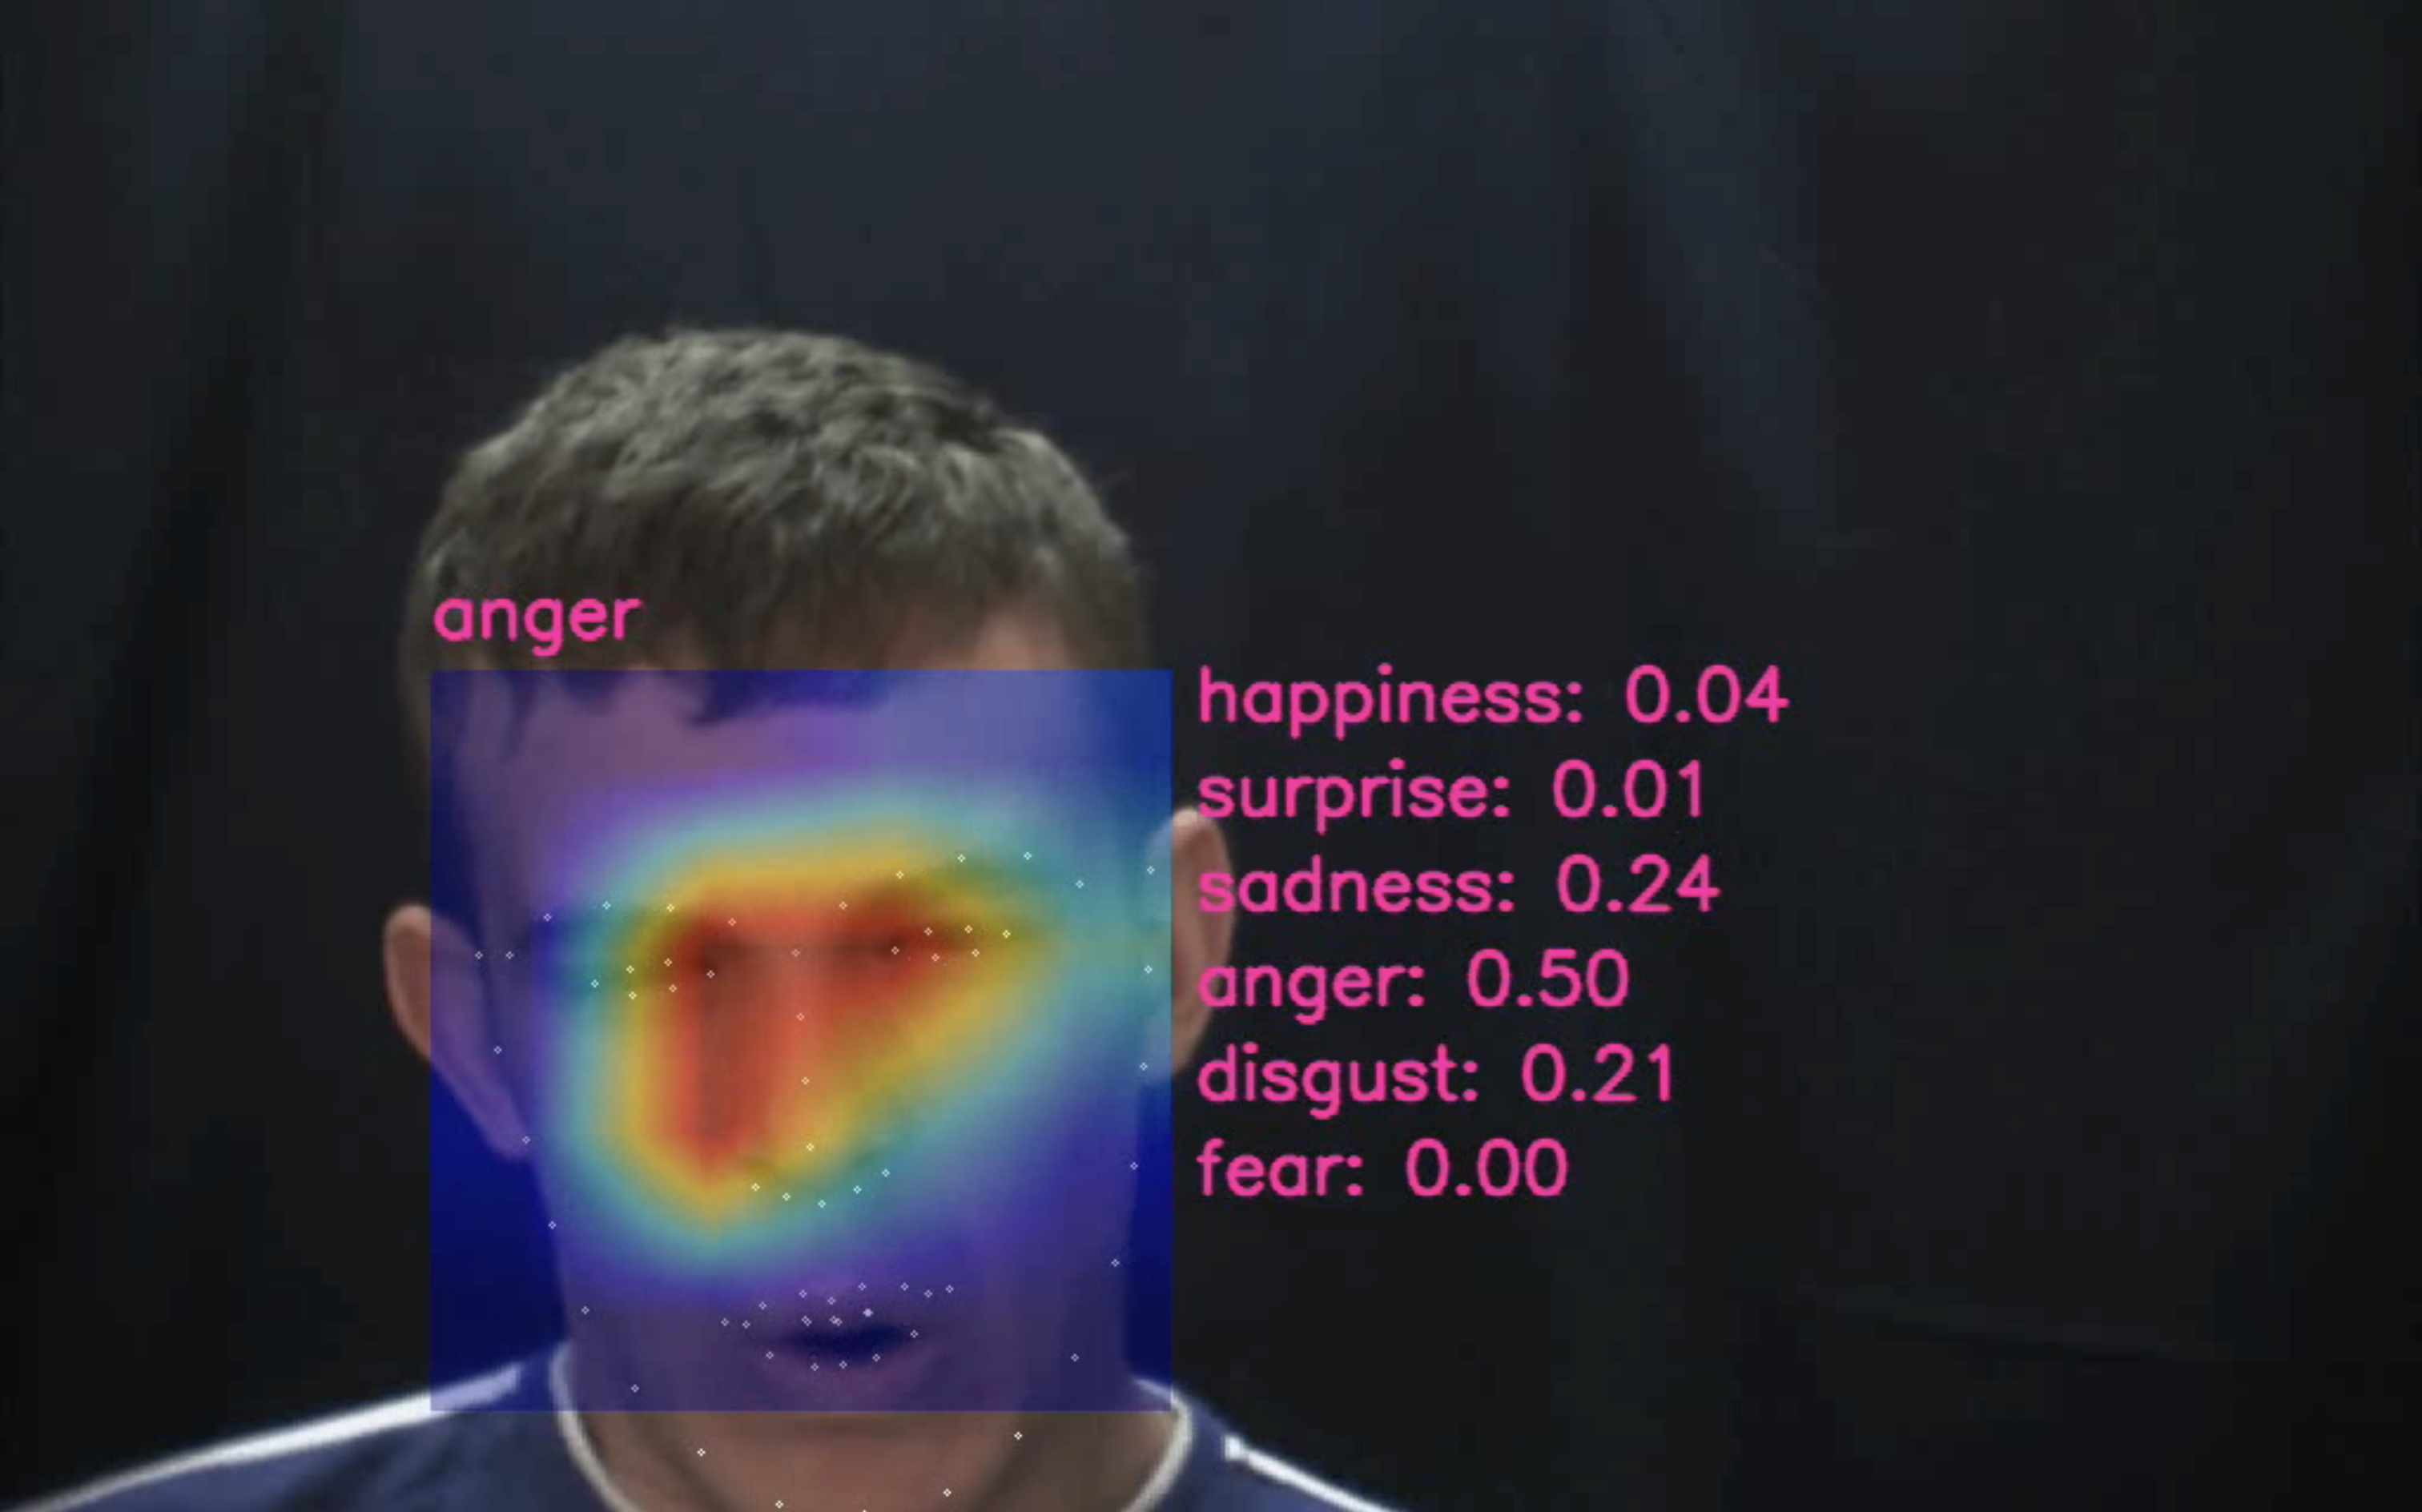
\includegraphics[width=\linewidth]{video/v_anger.png}
%     \caption{Sadness.}
%     \label{fig:v4}
%   \end{subfigure}
%   \hfill
%   \begin{subfigure}{0.32\linewidth}
%     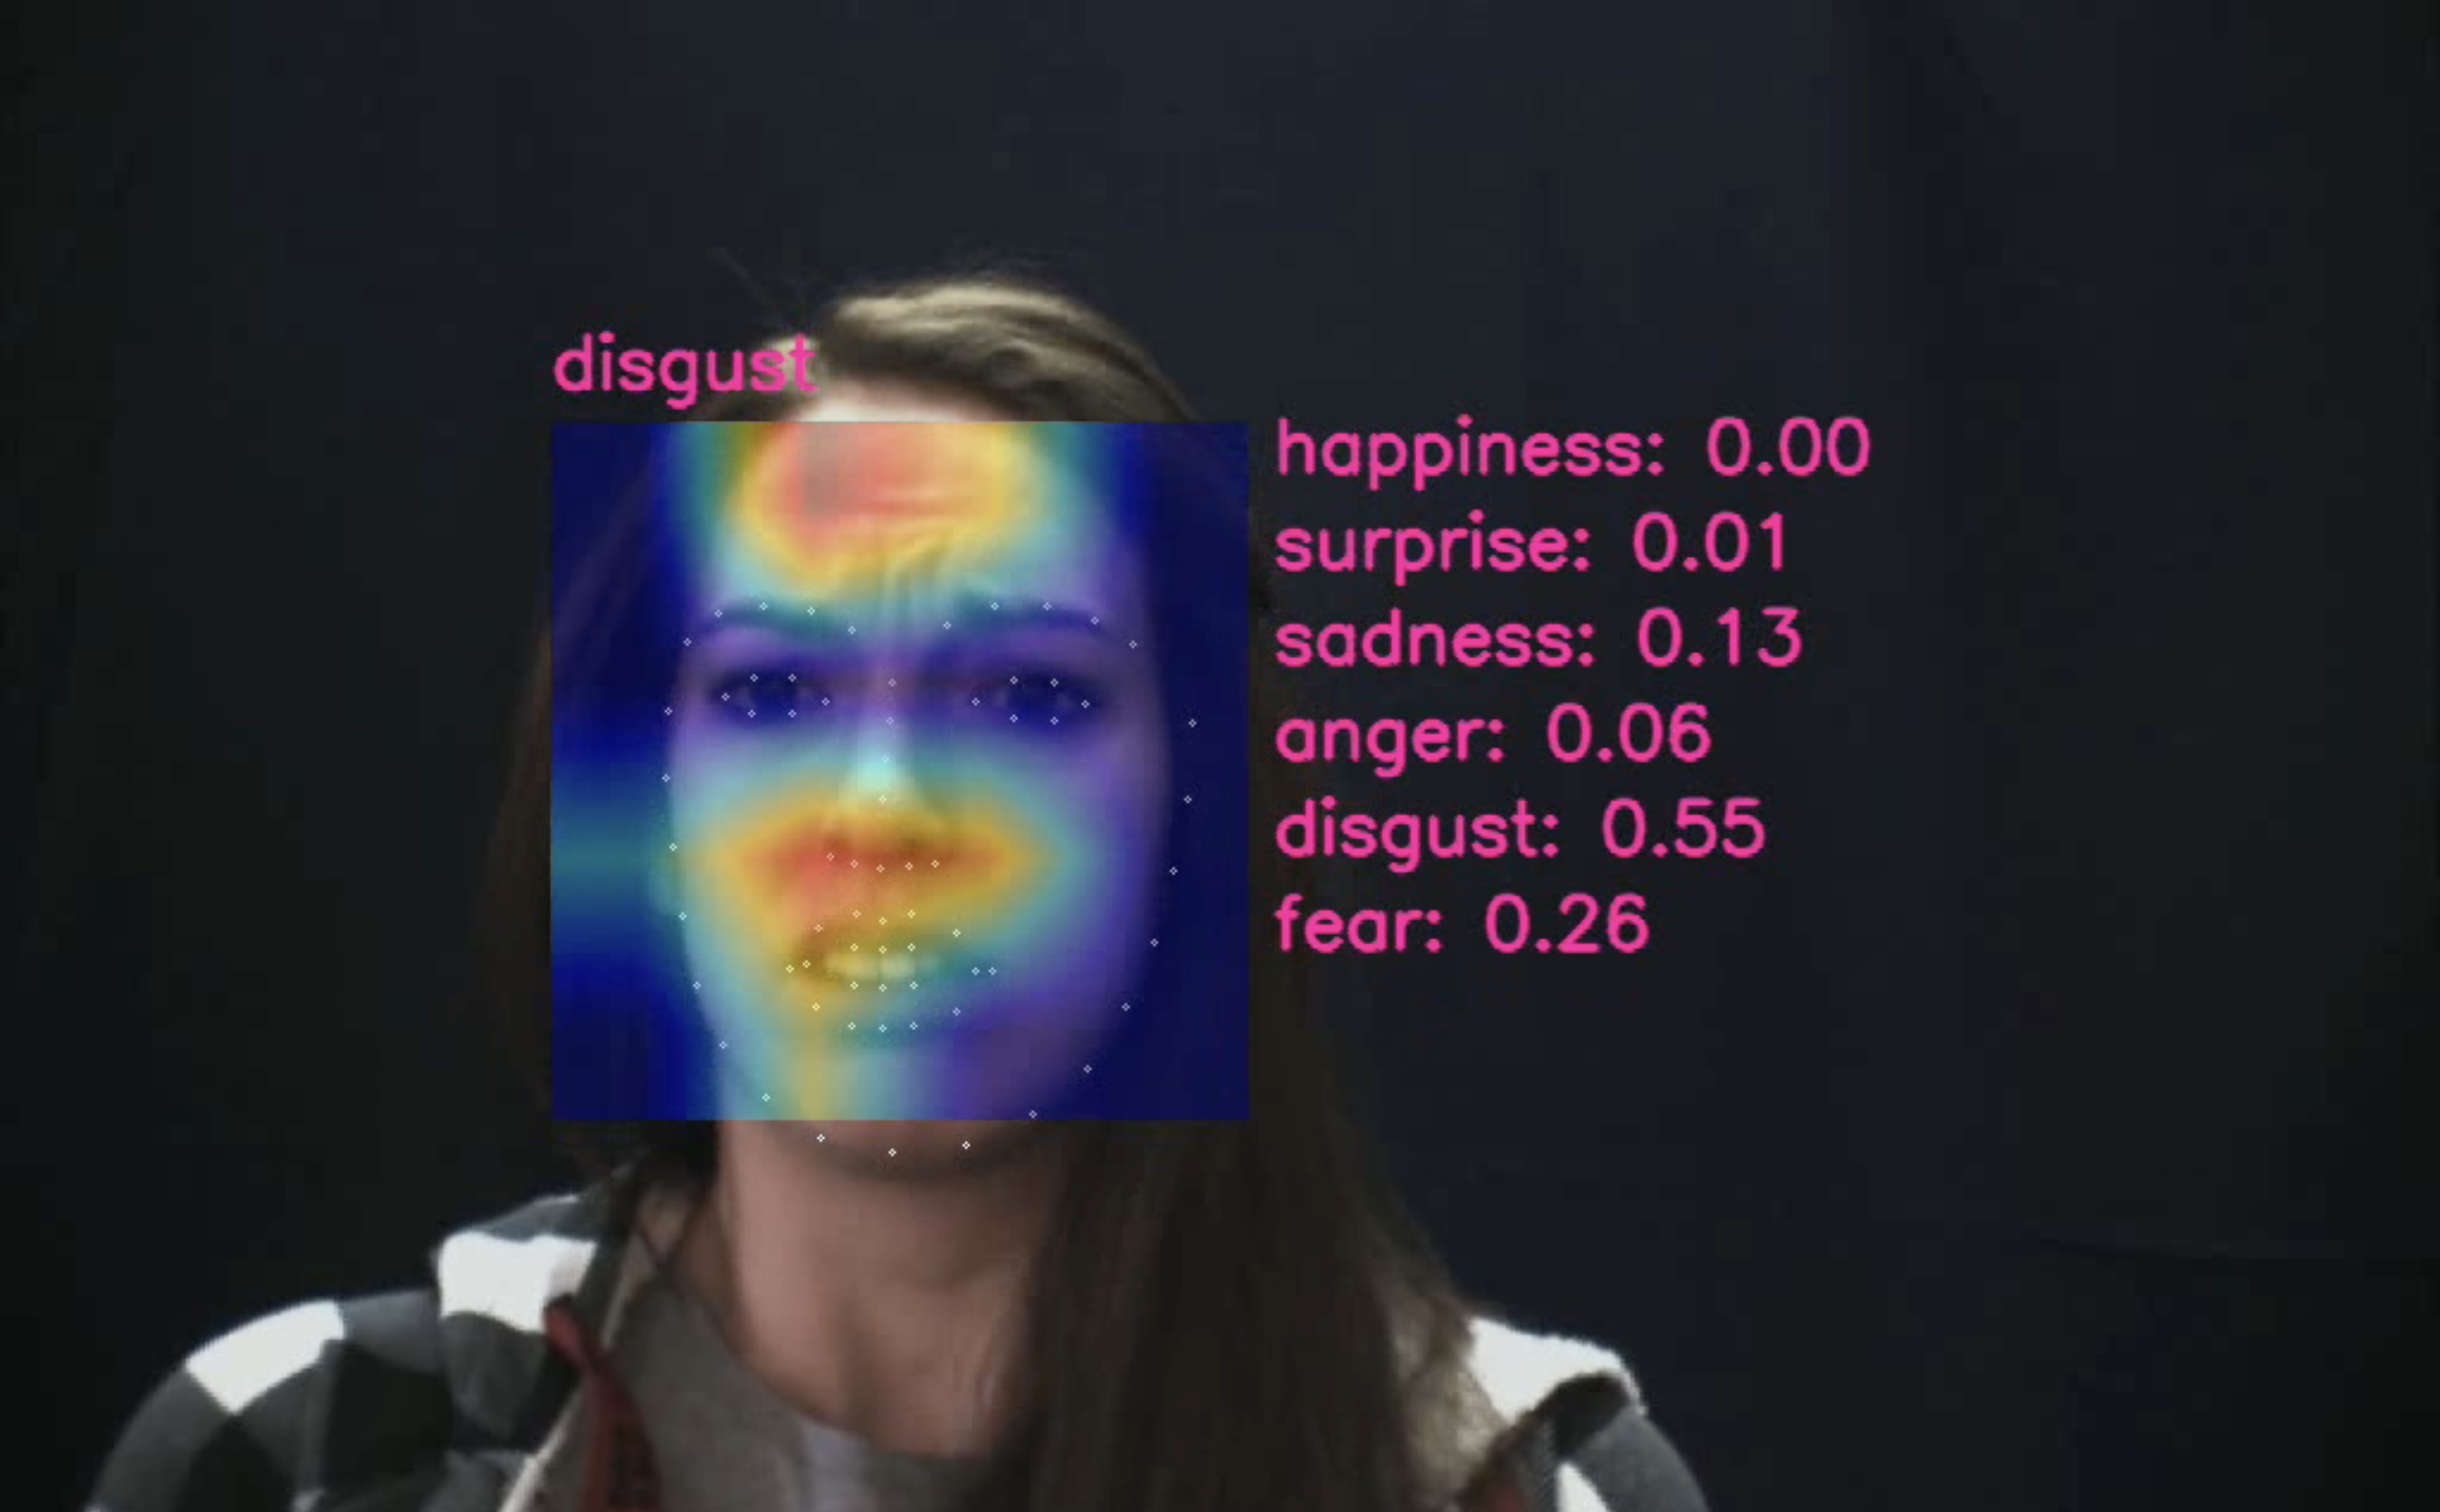
\includegraphics[width=\linewidth]{video/v_disgust.png}
%     \caption{Sadness.}
%     \label{fig:v5}
%   \end{subfigure}
%   \hfill
%   \begin{subfigure}{0.32\linewidth}
%     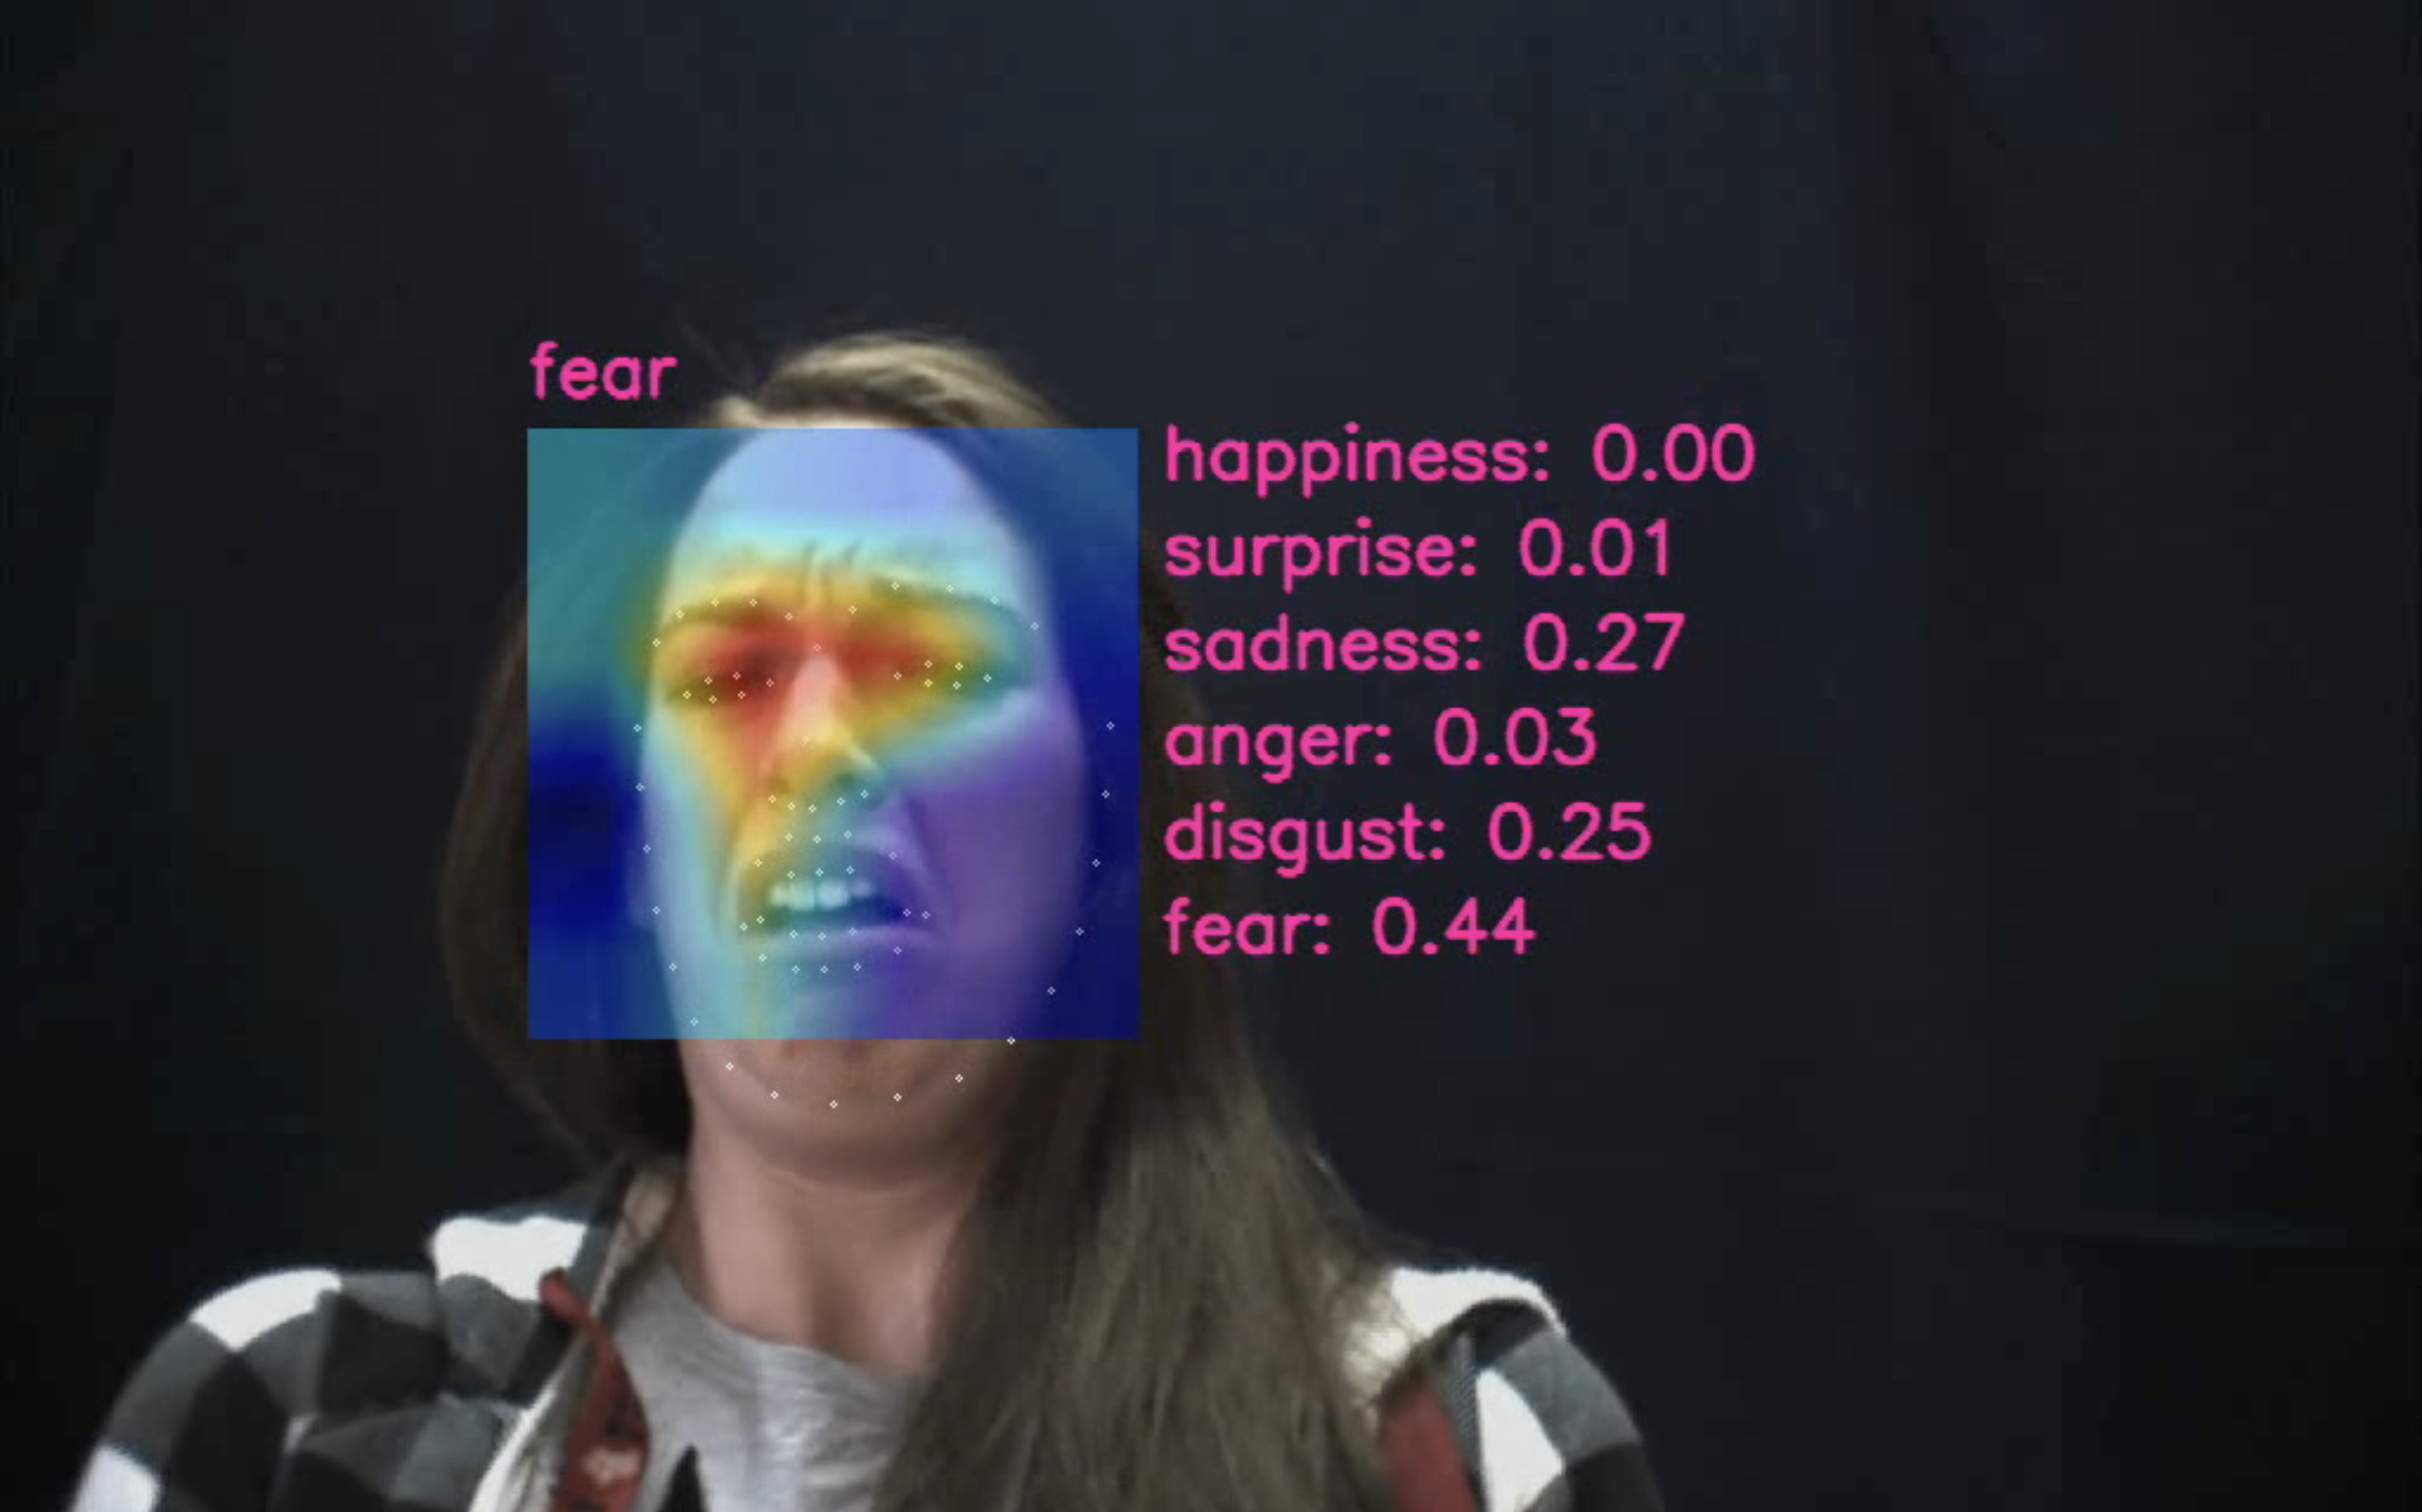
\includegraphics[width=\linewidth]{video/v_fear.png}
%     \caption{Sadness.}
%     \label{fig:v6}
%   \end{subfigure}
%   \hfill
%   \caption{Overview of XAI with grad-CAM and landmarks on DISFA dataset.}
%   \label{fig:video}
% \end{figure*}